\documentclass[landscape,a1paper,fontscale=0.5]{baposter}

% 9933 pixels x 14043 x 9933 pixels
%
% 
\includegraphics{images/cs_logo_colour.pdf}
%
%

\usepackage{graphicx, caption}
\usepackage{palatino}
\usepackage[font=scriptsize]{caption}

\definecolor{teal}{cmyk}{0.864, 0.443, 0.000, 0.655}
\definecolor{white}{cmyk}{0.00, 0.00, 0.00, 0.00}

\begin{document}
\begin{poster}
	{
    	grid=false,
        eyecatcher=true,
        background=none,
        columns=6,
        headershade=plain,
        headerColorOne=teal,
        headerFontColor=white,
        headerfont=\Large\textsf,
        headerborder=open,
        borderColor=teal,
        textborder=rectangle,
        boxshade=none
    }
	{
\includegraphics{images/cs_logo_colour.pdf}}
	{Map of the Internet}
	{Donald Martin}
	{
\includegraphics[width=2cm]{images/eyecatcher.png}}
    
    \headerbox{Motivation}{name=motivation, column=0,row=0, span=3}{
        The Internet is one of the most widely used man-made systems on the planet. So much
        so that former Microsoft CEO, Bill Gates, described the Internet as the ``\emph{town
        square for the village of tomorrow}.'' However, its inner workings are largely unknown
        to the vast majority of its users. Here, I will attempt to shed some light on the
        technical ingenuity behind the Internet.
    }
    
	\headerbox{Worldwide Connections}{name=worldwide_cxns, column=0, below=motivation, span=3}{
    	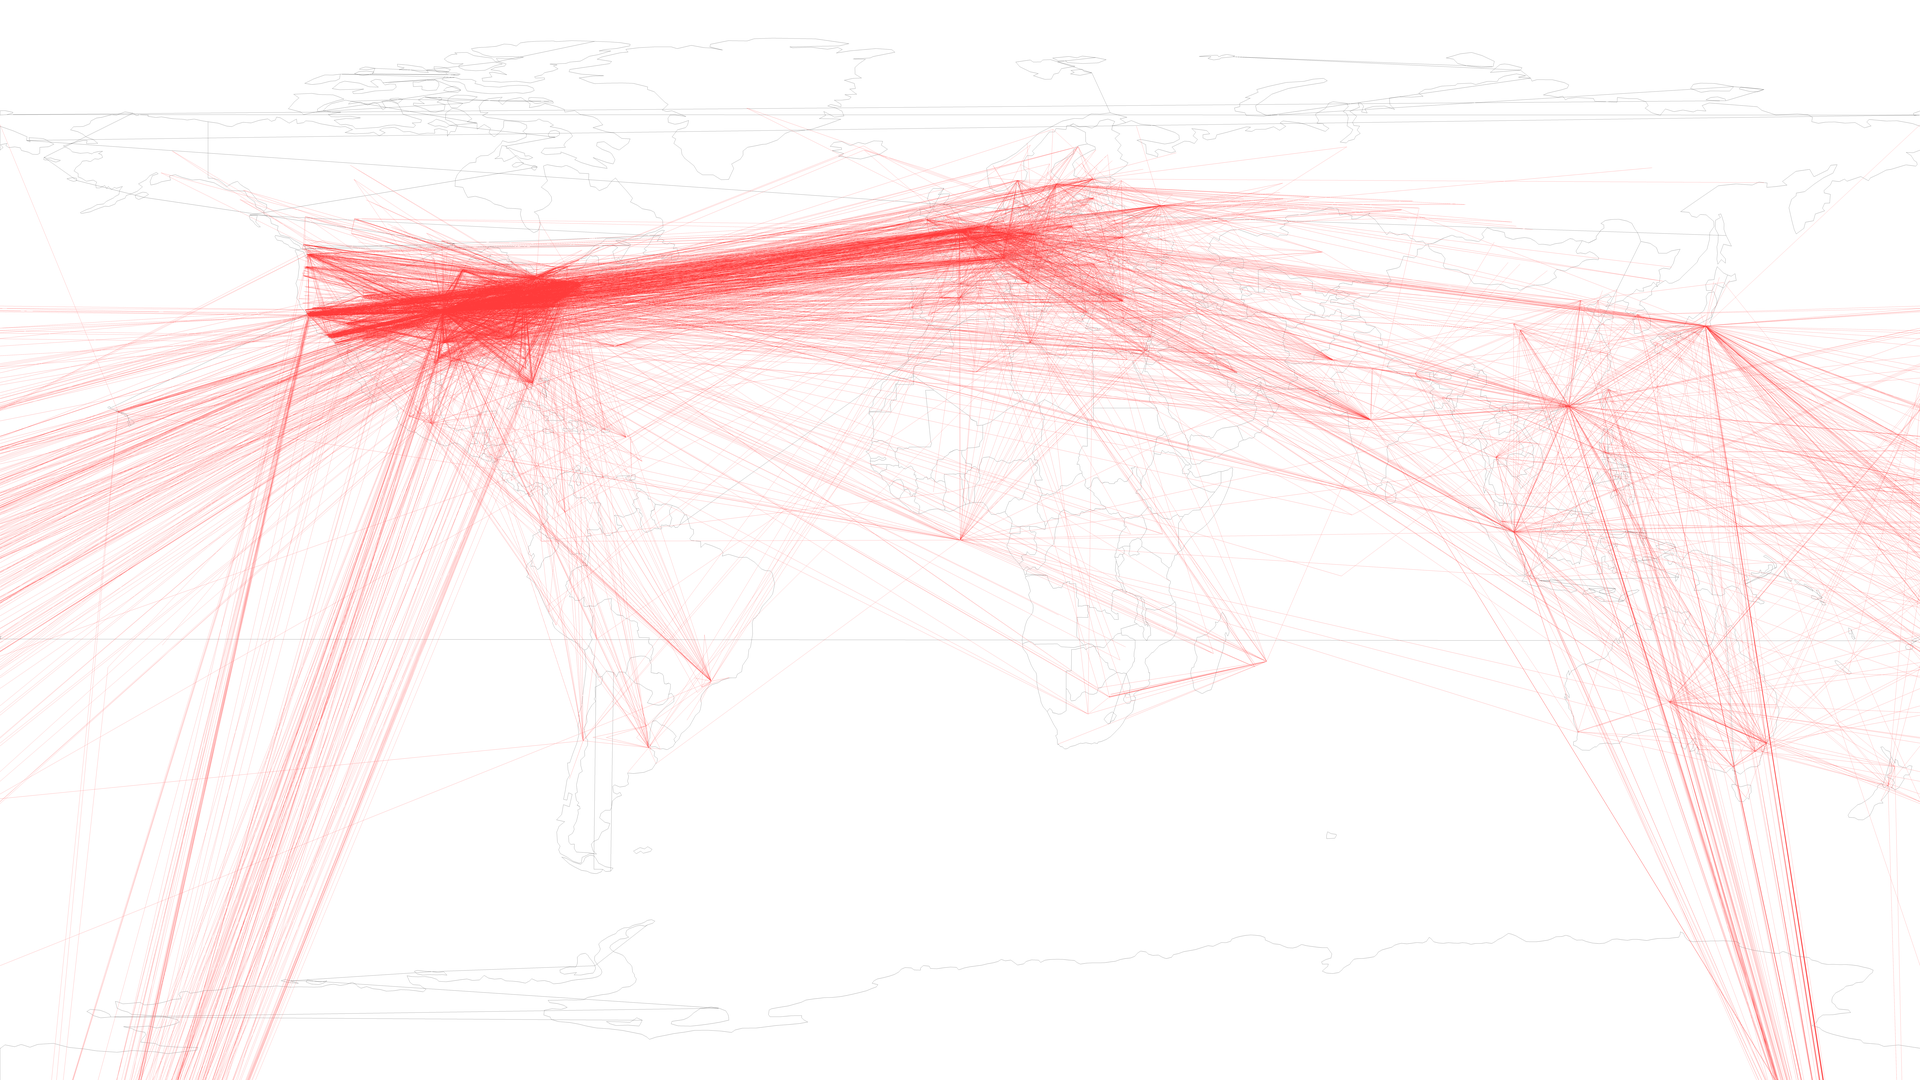
\includegraphics[width=\linewidth]{images/atlas.png}
        \captionof{figure}{Geographical Connections between Autonomous Systems}
        The Internet is foremost a large number of networks of computers working together. Each of these networks is an autonomous system (commonly, these are Internet Service Providers). Above, each autonomous system is represented as a point, based on the geographical location of its headquarters. Connections between autonomous systems are represented as lines. Here, we see a large number of transatlantic connections, showing the extent of Internet connectivity in the developed world, in contrast to Africa which has very few connections to other continents and even fewer autonomous systems.
    }
    
	\headerbox{The Need for IPv6}{name=need_for_ipv6, column=3,row=0, span=3}{
    	\begin{minipage}{0.33\linewidth}
            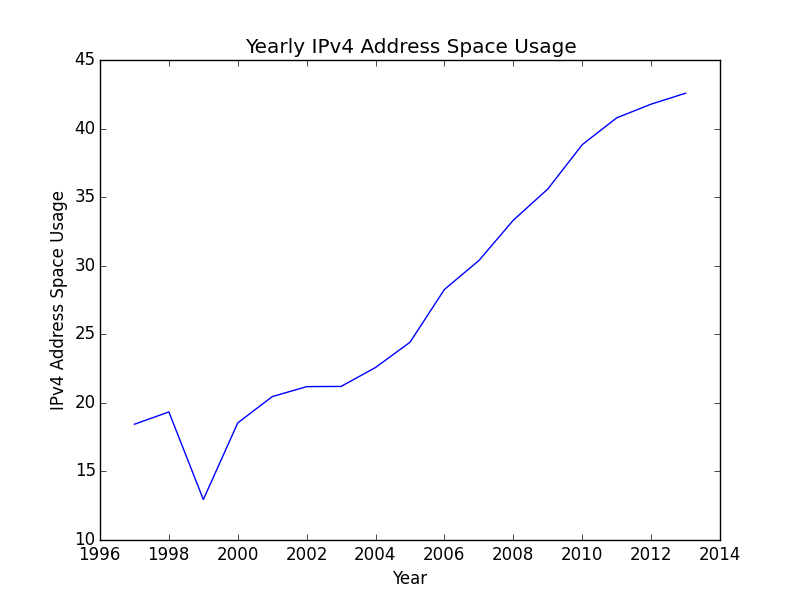
\includegraphics[width=\linewidth]{images/ipv4_address.png}
            \captionof{figure}{Yearly Visible Addresses}
        \end{minipage}
        \begin{minipage}{0.66\linewidth}
    		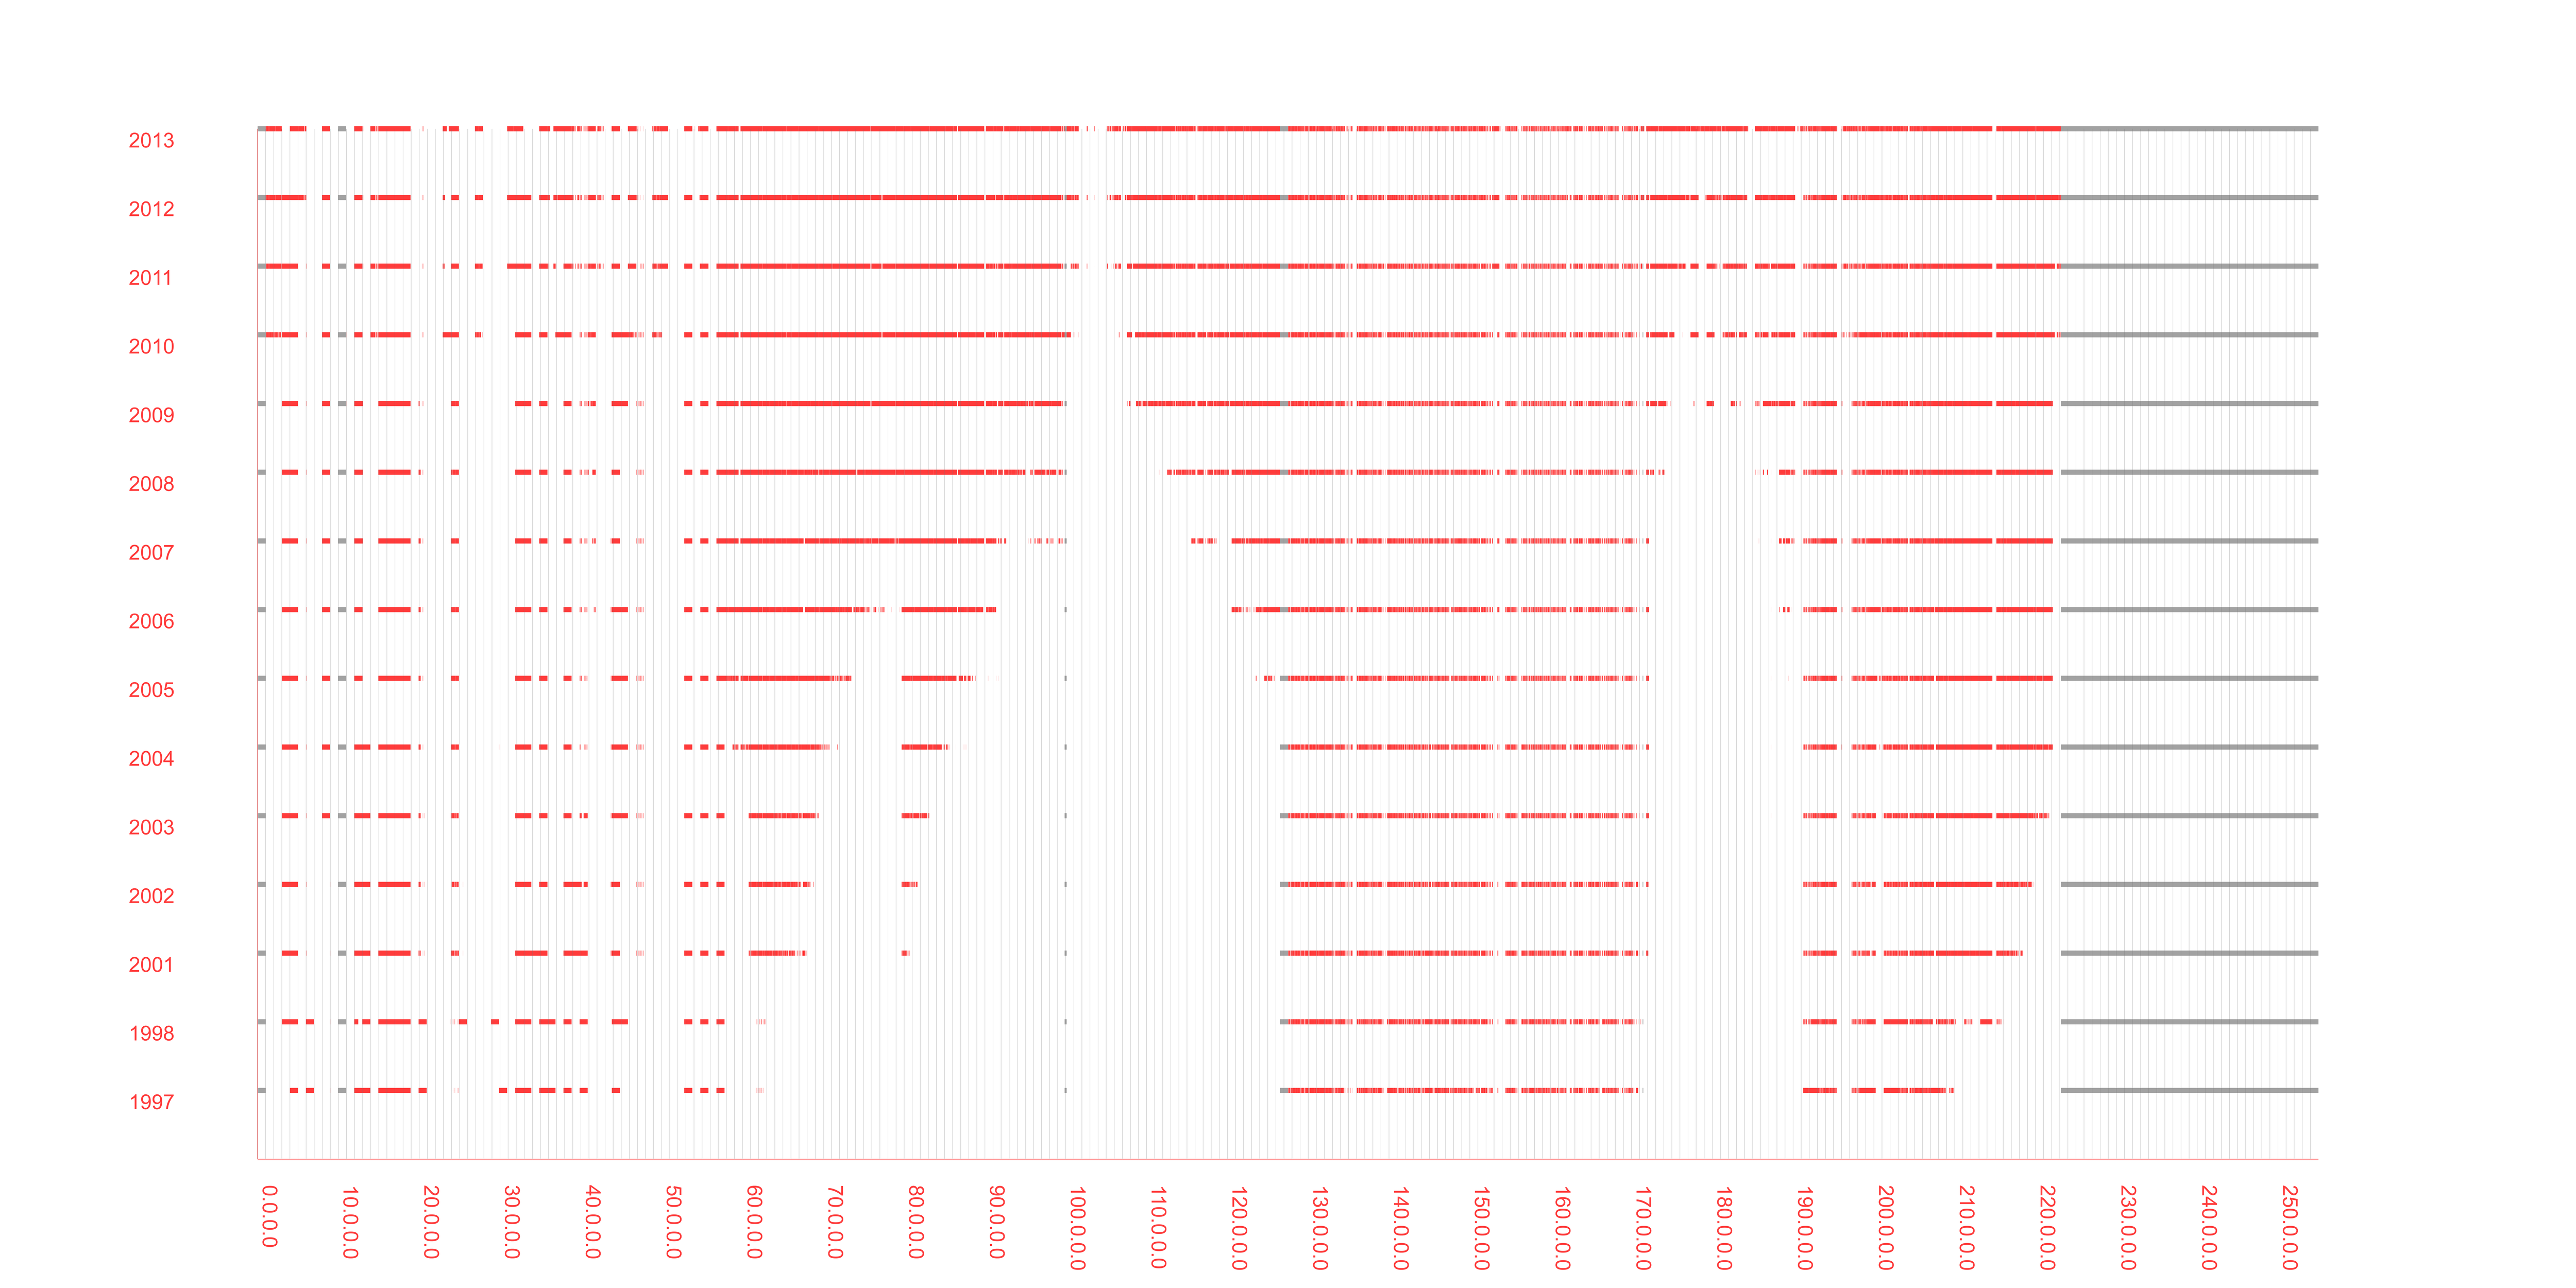
\includegraphics[width=\linewidth, height=4cm]{images/block_allocs.png}
            \captionof{figure}{Yearly IPv4 Addresses Used}
        \end{minipage}
  		IPv4 is the addressing system that is currently the most widely used
        on the Internet (how computers talk to each other). However, as IPv4
        is represented by 32 bits, the number of computers it can address is
        finite (a little over 4 billion computers). However, there are more
        than 7 billion people on the planet, many of whom have more than one
        device (for example, a mobile phone, a home computer, a work computer,
        etc).
        \\\\
        Currently, 45\% of all IPv4 space is visible to routers on the Internet,
        with 100\% of addresses having been allocated to regional registries for
        customer registration. As the graph on the left shows, the number of
        addresses visible on the network is largely linearly increasing, meaning
        that we can expect full saturation of the address space in the late 2020s.
        \\\\
        The graph on the right shows how the IPv4 address space is being used
        (grey represents addresses that cannot be allocated, such as broadcast
        and internal private addresses). As we can see, the address space is moving
        from the old classful system with three distinct blocks into a more
        continuous space after the introduction of classless addressing.
    }
    
    \headerbox{Internet Outages}{name=inet_outages, below=need_for_ipv6, column=3, span=3}{
    	\begin{minipage}{0.33\linewidth}
            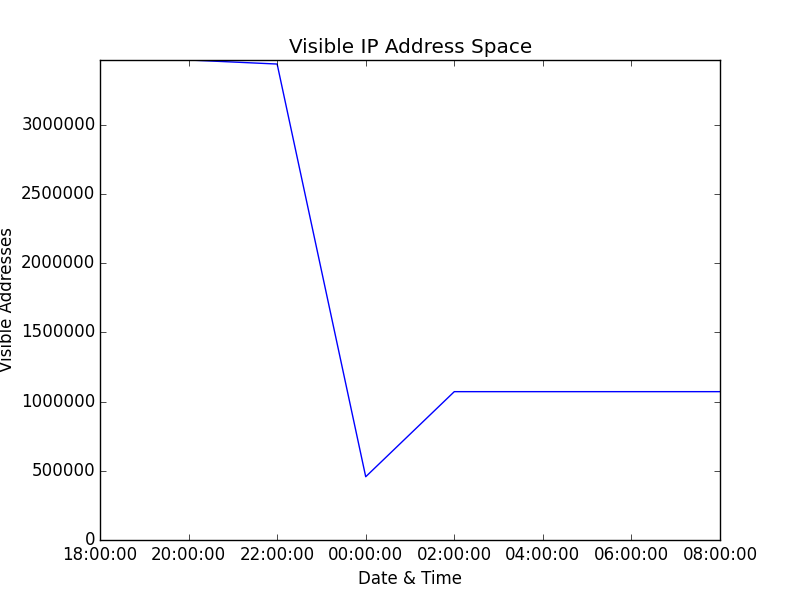
\includegraphics[width=\linewidth]{images/egypt-down.png}
            \captionof{figure}{Egyptian Visible Addresses}
        \end{minipage}
        \begin{minipage}{0.33\linewidth}
    		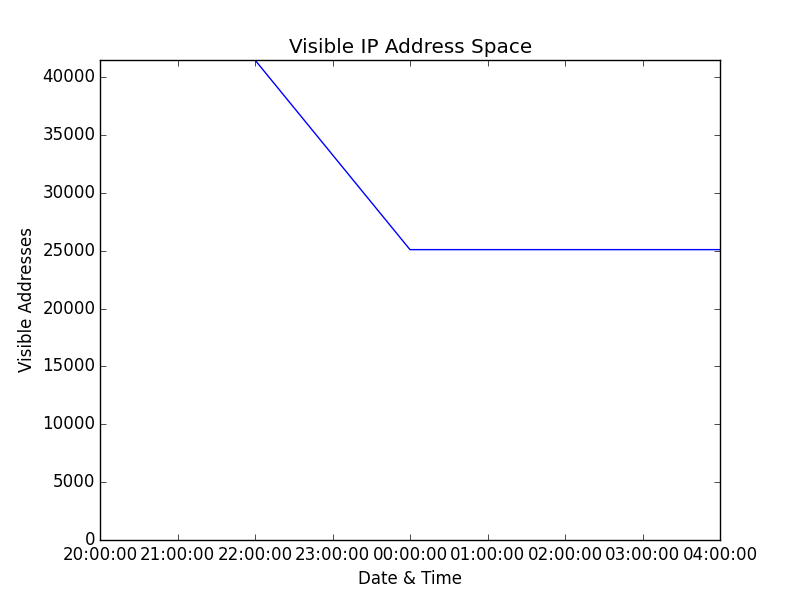
\includegraphics[width=\linewidth]{images/Libya_Drop-Off.png}
            \captionof{figure}{Libyan Visible IPv4 Addresses}
        \end{minipage}
    	\begin{minipage}{0.33\linewidth}
    		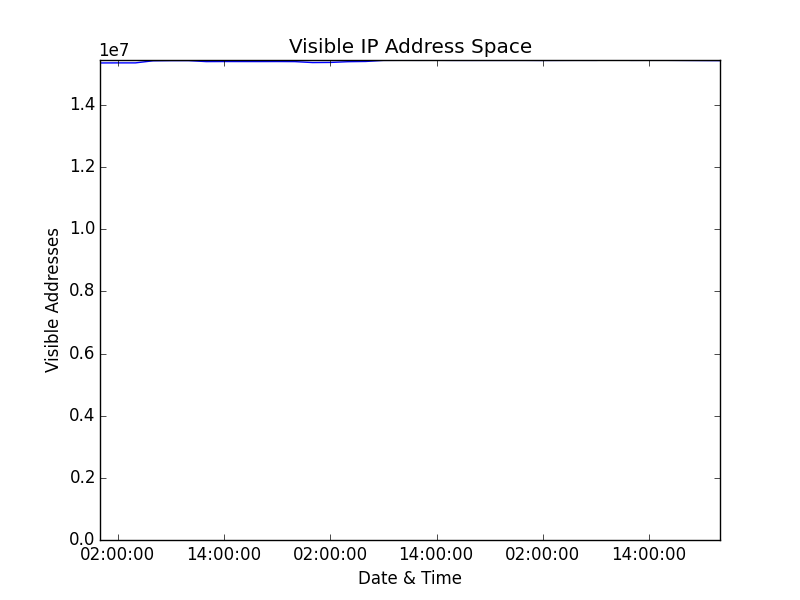
\includegraphics[width=\linewidth]{images/india.png}
            \captionof{figure}{Indian Visible IPv4 Addresses}
        \end{minipage}\\\\
        While new connections are actively broadcast between routers, so too
        are disconnections (route withdrawals). A route withdrawal is an
        indication that a connection is no longer available between two
        networks. While this disconnection may be caused by the end of a
        business relation, if we observe the network from various points, we
        can determine if a connection has been physically removed.
        \\\\
        Above are graphs showing the number of connections available to
        Egyptian networks during the 2011 Uprising, Libyan networks during
        the fall of Gaddafi and India following the cutting of an undersea
        cable in the Mediterranean.
        \\\\
        We can use this information to infer that Internet connectivity was
        forcibly removed in Egypt and Libya due to such a large percentage
        of networks losing connectivity to the outside world in under four
        hours. The remaining connections can be attributed to domestic ISP
        connections and/or errors in the GeoIP database used to map
        autonomous systems to countries.
    }
    
    \headerbox{Other Representations}{below=worldwide_cxns, column=0, span=3}{
    	\begin{minipage}{0.33\linewidth}
            \includegraphics[width=0.8\linewidth]{images/ring.png}
            \captionof{figure}{Networks positioned by Longitude}
        \end{minipage}
        \begin{minipage}{0.33\linewidth}
    		\includegraphics[width=0.8\linewidth]{images/staggered_ring.png}
            \captionof{figure}{More connected networks pulled in}
        \end{minipage}
        \begin{minipage}{0.33\linewidth}
			As with above, here we see autonomous systems represented as dots
            around the circumference of two circles, where the position of an
            AS is based on the longitude point on the above graph. This makes
            connections between Europe and North America easier to see, as
            they are more spread out than in the above geographical map.
            \\\\
            The circle on the right shows autonomous systems as dots based on
            their longitude around the circle, however, networks with more
            connections to other networks are pulled closer to the radius. 
           	Networks on the outside have only one connection, networks closer
            to the centre have more.
        \end{minipage}
    }
        
    \headerbox{Conclusions}{below=inet_outages, column=3, span=3}{
    	From the BGP routing information provided by the border gateway routers,
        it takes a very short length of time to determine if a large-scale
        incident has occurred in a foreign country. It is also clear that the
        current IPv4 addressing system is fast approaching capacity, and that the
        move to IPv6 is needed now more than ever.
    }
    

\end{poster}
\end{document}